
\section{Fairness-for-Event-B}
\label{sec:Fairness-for-Event-B}
\newcommand{\WF}{\mathrm{WF}}
\newcommand{\SF}{\mathrm{SF}}
\newcommand{\RESP}[2]{#1\rightsquigarrow{#2}}
\subsection{Introduction}
Fairness is a property for system which have infinite execution, this property ensure that transitions (events) can be "fairly" chosen to execute when their preconditions (guards) are satisfied. Without fairness constraints, it's possible that some transitions can be always ignored even if they are enabled in some states. It does not make sense to deal with fairness constraints on systems with finite execution.
\paragraph{Weak Fairness}
% K1: none of this makes sense. WF(t) is a quality of an execution (and a transition set t)
% K2: this is not right yet. You cannot talk rigorously about fairness without given an explicit definition of an execution. FIXME
An transition set t is a weakly fair set if every transition in t is always eventually disabled or infinitely often taken.
\begin{displaymath}
  \WF(i)\Equiv\Always\Eventually\Not g_i\Or\Always\Eventually\mathrm{taken}_i
\end{displaymath}
\paragraph{Strong Fairness}
An transition set t is a strongly fair set if every transition in t is eventually always disabled or infinitely often taken.
\begin{gather*}
  \SF(i)\Equiv\Eventually\Always\Not g_i\Or\Always\Eventually{\mathrm{taken}}_i
\end{gather*}
However, by working on the definitions for weak fairness and strong fairness, we can easily find that strong fairness imply weak fairness. Strong fairness is stronger than weak fairness.  
% K2: you may want to introduce a notation \sigma\models\phi to express that formula \phi (eg WF(i)) holds in execution \sigma. This is just standard LTL semantics.
\begin{gather*}
  \SF(i)\Implies \WF(i)
\end{gather*}

\paragraph{Event Merging}
% K2: this doesn't work yet. First introduce the two events for plane and train travel, then discuss WF for the group. I don't think you need a name for the group event.
For some situations we only have the fairness constraints for a set of events instead of fairness constraints for each of them. For example, Peter wants to travel all over the world, once he arrives at a new place, he might stay there and spend several days for sightseeing, and he can only take train or aiplane to travel. In this example, assume having an one-day sightseeing is modeled as the event $E_{\mathrm{sightseeing}}$, the event $E_{\mathrm{air}}$ is for moving on air and the event $E_{\mathrm{train}}$ is for moving by train. We also introduce an event $E_{\mathrm{air}\Or\mathrm{train}}$, which is an event moving to another place either on air or by train.\\
\\
\usetikzlibrary{arrows}
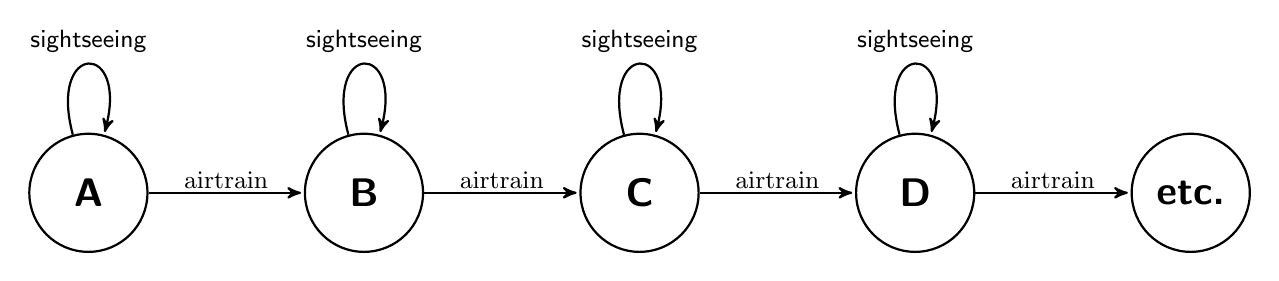
\begin{tikzpicture}[->,>=stealth',shorten >=1pt,auto,node distance=3.5cm,
  thick,main node/.style={circle,fill=white!20,draw,
  font=\sffamily\Large\bfseries,minimum size=15mm}]

  \node[main node] (A) {A};
  \node[main node] (B) [right of=A] {B};
  \node[main node] (C) [right of=B] {C};
  \node[main node] (D) [right of=C] {D};
  \node[main node] (E) [right of=D] {etc.};

  \path[every node/.style={font=\sffamily\small,
  		fill=white,inner sep=1pt}]
  	% Right-hand-side arrows rendered from top to bottom to
  	% achieve proper rendering of labels over arrows.
    (A) edge [loop above] node[above=1mm] {sightseeing} (A)
        edge node {$\mathrm{air}\Or\mathrm{train}$} (B)
        
    (B) edge [loop above] node[above=1mm] {sightseeing} (B)
        edge  node{$\mathrm{air}\Or\mathrm{train}$} (C)
    (C) edge [loop above] node[above=1mm] {sightseeing} (C)
        edge node{$\mathrm{air}\Or\mathrm{train}$} (D)
    (D) edge [loop above] node[above=1mm] {sightseeing} (D)
        edge node{$\mathrm{air}\Or\mathrm{train}$} (E) ;
   
\end{tikzpicture}
\\
\\
The following constraint
\begin{displaymath}
  \WF(air\Or{train})
\end{displaymath}
must be satisfied to ensure he does move from one place to another rather than spending the rst of his life sightseeing somewhere without ever moving again.\\
\\
\usetikzlibrary{arrows}
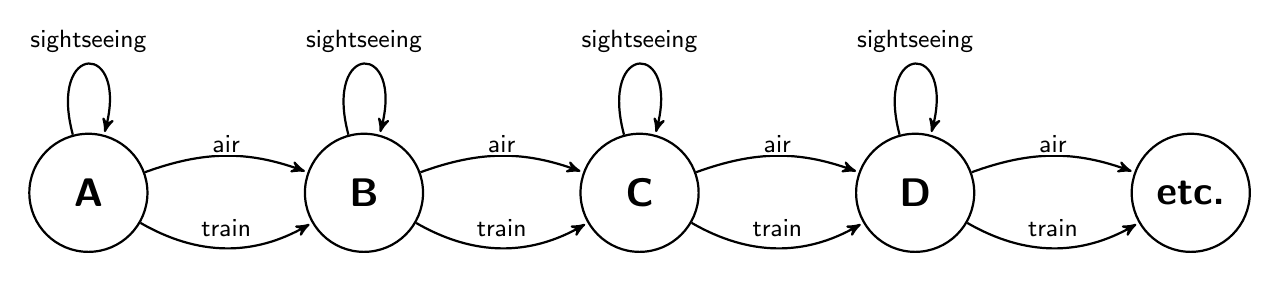
\begin{tikzpicture}[->,>=stealth',shorten >=1pt,auto,node distance=3.5cm,
  thick,main node/.style={circle,fill=white!20,draw,
  font=\sffamily\Large\bfseries,minimum size=15mm}]

  \node[main node] (A) {A};
  \node[main node] (B) [right of=A] {B};
  \node[main node] (C) [right of=B] {C};
  \node[main node] (D) [right of=C] {D};
  \node[main node] (E) [right of=D] {etc.};

  \path[every node/.style={font=\sffamily\small,
  		fill=white,inner sep=1pt}]
  	% Right-hand-side arrows rendered from top to bottom to
  	% achieve proper rendering of labels over arrows.
    (A) edge [loop above] node[above=1mm] {sightseeing} (A)
        edge [bend left=20] node {air} (B)
        edge [bend right=30]node[above=1mm] {train}(B)
    (B) edge [loop above] node[above=1mm] {sightseeing} (B)
        edge [bend left=20] node{air} (C)
        edge [bend right=30]node[above=1mm] {train}(C)
    (C) edge [loop above] node[above=1mm] {sightseeing} (C)
        edge [bend left=20] node{air} (D)
        edge [bend right=30]node[above=1mm] {train}(D)
    (D) edge [loop above] node[above=1mm] {sightseeing} (D)
        edge [bend left=20] node{air} (E) 
        edge [bend right=30]node[above=1mm] {train}(E);
   
\end{tikzpicture}
\\
\\
If every place has an airport and a train station, or none of them, travel is fair (can be always eventually chosen) iff air is fair (can be always eventually chosen) or train is fair (can be always eventually chosen). Since if one of the transportations is fair to choose, he can always eventually move to other places.
\begin{displaymath}
  \mathrm{I}\And{g_{air}} = \mathrm{I}\And{g_{train}}\Implies(\WF(air\Or{train})\Equiv\WF(air)\lor\WF(train))
\end{displaymath}
However, if there have at least one place that has only have airport, $\WF(train)$ can't ensure he can leave this place unless there have extra requirements force him occationally move on air (weak fairness for air when train is disabled). We also have similar problem for places only have train station. \\
\\
\usetikzlibrary{arrows}
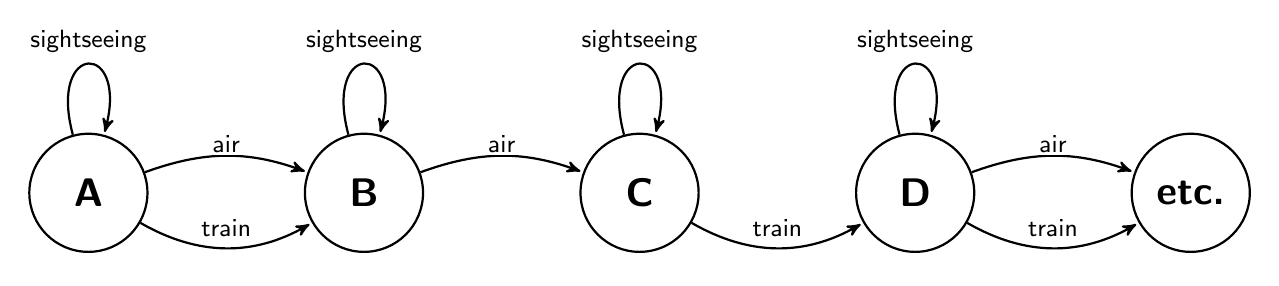
\begin{tikzpicture}[->,>=stealth',shorten >=1pt,auto,node distance=3.5cm,
  thick,main node/.style={circle,fill=white!20,draw,
  font=\sffamily\Large\bfseries,minimum size=15mm}]

  \node[main node] (A) {A};
  \node[main node] (B) [right of=A] {B};
  \node[main node] (C) [right of=B] {C};
  \node[main node] (D) [right of=C] {D};
  \node[main node] (E) [right of=D] {etc.};

  \path[every node/.style={font=\sffamily\small,
  		fill=white,inner sep=1pt}]
  	% Right-hand-side arrows rendered from top to bottom to
  	% achieve proper rendering of labels over arrows.
    (A) edge [loop above] node[above=1mm] {sightseeing} (A)
        edge [bend left=20] node {air} (B)
        edge [bend right=30]node[above=1mm] {train}(B)
    (B) edge [loop above] node[above=1mm] {sightseeing} (B)
        edge [bend left=20] node{air} (C)
    (C) edge [loop above] node[above=1mm] {sightseeing} (C)
        edge [bend right=30]node[above=1mm] {train}(D)
    (D) edge [loop above] node[above=1mm] {sightseeing} (D)
        edge [bend left=20] node{air} (E) 
        edge [bend right=30]node[above=1mm] {train}(E);
   
\end{tikzpicture}
\\
\\
We have:
\begin{displaymath}
  (\WF(train)\And\WF(air@g_{air}\And\Not{g}_{train}))\Or(\WF(air)\And\WF(train@g_{train}\And\Not{g}_{air})) \Equiv\WF(t)
\end{displaymath}
For this type of constraints, we introduce the following rule for
merging events: For event $E_{i}$ and event $E_{j}$, where $i,j \in$
I, the merged event $E_{i\Or j}$ is given as:
\begin{align*}
g_{i\Or {j}} & =  g_i\Or g_j\\
a_{i\Or {j}} & |  a'_{i\Or j} \And \\
           &    (((g_i\And\Not g_j)\Implies (a'_{i\Or j} = a_i))\\
           &    \Or ((\Not g_i\And g_j)\Implies (a'_{i\Or j} = a_j))\\
           &    \Or ((g_i\And g_j)\Implies (a'_{i\Or j} = a_j\Or a_j)))
\end{align*}
The merged event $E_{i\lor{j}}$ can happen whenever either of its constituent events ($E_i$ and $E_j$) could fire, and if $E_{i\lor{j}}$ fires, the effect is one of the enabled constituent events.\\
Some properties for fairness constraints of merged events are:\\
Assume $i,j \in$ I, event $E_{i\Or j}$ is the result of merging events $E_i$ and $E_j$.
\begin{gather*} 
  (\WF(i)\And\WF(j@g_{j}\And\Not{g}_{i}))\Or(\WF(j)\And\WF(i@g_{i}\And\Not{g}_{j})) \Equiv\WF(i\Or{j})\\
  (\SF(i)\And\SF(j@g_{j}\And\Not{g}_{i}))\Or(\SF(j)\And\SF(i@g_{i}\And\Not{g}_{j})) \Equiv\SF(i\Or{j})
\end{gather*}

\paragraph{Event Splitting}
In an opposite way, we can also split an event into two mutually exclusive sub-events, by refining them with different mutually exclusive strengthened guards which imply the original guard. \\
For event $h$ where $h \in I$, event $i$ and event $j$ are \emph{split} events of $h$ iff:
\begin{gather*} 
g_i \Or g_j \Equiv g_h\\
\Not(g_i\And g_j)\\
a_i = a_j = a_h
\end{gather*}
Note that the fairness constraints of the original event are not inherited to its sub-events, for the same reason explained in event merging part.
However, similar to the outcome of the event merging process, we can say a event is fair if we can ensure that one of its sub-events is fair, since the sub-events have same guard as the original event.
\begin{gather*} 
  \WF(i) \Or \WF(j) \Implies  \WF(h)\\
  \SF(i) \Or \SF(j) \Implies \SF(h)
\end{gather*}
Where event $i$ and $j$ are sub-events of event $h$.\\\\
Currently Event-B does not have suppport for LTL, most of properties described by LTL (including fairness) can't be assumed or proved by Event-B. In the rest parts of this report, we will extend the original Event-B method and show the usage of fairness assumptions for proving response properties.\\

%====================
\subsection{The Extended Event-B method}
We need to make several modifications to support fairness and other properties defined in LTL. We need to ensure that the machine have infinite executions and add an area to store LTL related assumptions.
\paragraph{Infinite execution}
To ensure the infinite execution for a machine, the only thing we need to check that there is always at least one event (except event $E_0$) is enabled to be executed, i.e., the invariants $J$ always satisfy at least one guards of events in $I_1$. We introduce the theorem $thm_{InfExe}$ for infinite execution:\\
\begin{displaymath}
  \bigvee_{i\in{I_1}}^{} g_i
\end{displaymath}
If $thm_{InfExe}$ keep holding, always at least one event can be executed.\\

\paragraph{Assumptions}
After ensuring the infinite execution, we also introduce a new part in the machine, called  \texttt{Assumptions}, which store the LTL based assumptions.\\
For event $i$ where $i\in{I_1}$, available assumptions are:\\
Weak Fair:
\begin{displaymath}
  \WF(i)
\end{displaymath}
and Strong Fair:
\begin{displaymath}
  \SF(i)
\end{displaymath}
and Response:
\begin{displaymath}
  \RESP{p}{q}
\end{displaymath}

For state p and q, available assumption
where $i\in{I_1}$, and $p$ and $q$ are states. Details about response property are in the next section.

\subsection{Proving rules for response properties in Extended Event-B}
Response property describes a relationship between two states $p$ and $q$, we say $\RESP{p}{q}$ iff $q$ will always eventually happen once after $p$ happened. 
\begin{displaymath}
  \RESP{p}{q}\Equiv({p}\Implies\Eventually{q})
\end{displaymath}
Response have following general properties:\\
Reflexivity:
\begin{displaymath}
  \RESP{a}{a}
\end{displaymath}
Transitivity:
\begin{displaymath}
  \frac{\RESP{p}{q},\RESP{q}{r}}{\RESP{p}{r}}
\end{displaymath}
Monotonicity:
\begin{displaymath}
  \frac{p\Implies{p'},\RESP{p'}{q'},q'\Implies{q}}{\RESP{p}{q}}
\end{displaymath}
Disjunction:
\begin{displaymath}
  \frac{\RESP{p}{r},\RESP{q}{r}}{\RESP{{(p\Or{q}})}{r}}
\end{displaymath}
In addition, we need rules for specific situations. Before applying following rules, we assume the $thm_{InfExe}$ and Event-B usual POs have been proved already.
\paragraph{Proof rule for the only events}
For state $p$, we say event $E_{i}$ is the only event for $p$, written ($\mathrm{Only}_{i}({p})$), if at state $p$, event $i$ is the only event enabled.
\begin{gather*}
  i\in{I_1} \\
  p\in{J}\And{g_{i}} \\
  \frac{p\notin{J}\And\bigvee_{j\in({I_1}\setminus\{{i}\})}^{} g_{j}}{\mathrm{Only}_{i}({p})}
\end{gather*}
We introduce the Only set, $\mathrm{Only}({i})$, which satisfy
\begin{displaymath}
  \mathrm{Only}_{i}({p})\Equiv{p}\in\mathrm{Only}({i})
\end{displaymath}
where for all $i\in{I_0}$
\begin{displaymath}
  \mathrm{Only}({i}) = {J}\And{g_{i}}\And\bigvee_{j\in({I_1}\setminus\{{i}\})}^{} g_{j}
\end{displaymath}

\usetikzlibrary{arrows}
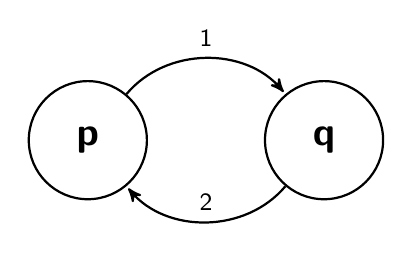
\begin{tikzpicture}[->,>=stealth',shorten >=1pt,auto,node distance=3cm,
  thick,main node/.style={circle,fill=white!10,draw,
  font=\sffamily\Large\bfseries,minimum size=15mm}]

  \node[main node] (p) {p};
  \node[main node] (q) [right of=p] {q};

  \path[every node/.style={font=\sffamily\small,
  		fill=white,inner sep=1pt}]
  	% Right-hand-side arrows rendered from top to bottom to
  	% achieve proper rendering of labels over arrows.
    (p) 
        edge [bend left=50] node[above=1mm] {1} (q)
    (q) 
        edge [bend left=50] node[above=1mm] {2} (p);
 
\end{tikzpicture}\\
An example is a machine presented by graph above. In this machine, event 1 is the only event at state $p$ and event 2 is the only event at state $q$, $\mathrm{Only}(1) = {p}$ and $\mathrm{Only}(2) = {q}$.\\
Now we want to prove $\RESP{p}{q}$.\\
Since at state $p$ we can choose event 1 only, which will move from $p$ to $q$ directly, so that $q$ must be the next state after $p$, which satisfies $\RESP{p}{q}$.
\begin{displaymath}
  \mathrm{Only}_{i}({p})\And({p}\And{a_{i}} = {q'}) 
  \Implies({p}\Implies\Next{q})
  \Implies({p}\Implies\Eventually{q})
  \Equiv{\RESP{p}{q}}
\end{displaymath}
In general, we have rule \texttt{$\mathrm{RESP_{ONLY}}$}
\begin{gather*}
  \mathrm{Only}_{i}({p})\\
  \frac{{J}\And{g_{i}}\And{p}\And{a_{i}} = {q'}}{\RESP{p}{q}}
\end{gather*}
\paragraph{Proof rule for the weakly fair events}
%X:need cite
Manna and Pnueli had present a proved single-step rule to validate response properties under weak fairness assumption for the helpful transition. Their rule is:
\begin{gather*}
  p\Implies({q}\Or\varphi)\\
  \forall{\tau}\in{T}(\rho_{\tau}\And\varphi)\Implies({q'}\Or\varphi')\\
  (\rho_{\tau_{h}}\And\varphi)\Implies{q'}\\
  \frac{\varphi\Implies({q}\Or\mathrm{En(\tau_{h})})}{\RESP{p}{q}}
\end{gather*}
where $T$ is the set of transitions, $\tau_{h}$ is the helpful transition, $\mathrm{En(\tau_{h})}$ is the precondition enable $\tau_{h}$ to be taken and $\rho_{\tau}$ is the after state for transition $\tau$.\\
In Event-B, the transition set $T$ can be represented by the events set $I_1$, the helpful transition $\tau_{h}$ can be represented by the helpful event $h$, the precondition $\mathrm{En(\tau_{h})}$ can be represented by $J\And{g_{h}}$, and the after state $\rho_{\tau}$ can be represented by $J\And{g_(i)}\And{a_{i}}$. By replacing $\varphi$ by $\phi$, the Event-B version of the rule (\texttt{$\mathrm{RESP_{WF}}$}) is:
\begin{gather*}
  {J}\And{p}\Implies{q}\And\phi\\
  \forall{i}\in{I_1}({J}\And{g_{i}}\And{a_{i}}\And\phi\Implies{q'}\Or\phi')\\
  \WF(h)\\
  {J}\And{g_{h}}\And{a_{h}}\And\phi\Implies{q'}\\
  \frac{{J}\And\phi\Implies{q}\Or{g_{h}}}{\RESP{p}{q}}
\end{gather*}
\paragraph{Proof rule for the strongly fair events}
The single-step rule for strong fairness is similar to the one for weak fairness. However, if a helpful event {h} is strongly fair, we only need ${J}\And\phi\Implies\Eventually({q}\Or{g_{h})}$, instead of ${J}\And\phi\Implies{q}\Or{g_{h}}$, since $\SF(h)$ ensure ${h}$ can be eventually chosen if $\Eventually{g_{h}}$ applies. \\
From the definition of response, we have
\begin{gather*}
  {J}\And\phi\Implies\Eventually({q}\Or{g_{h})}\\
  \Equiv\\
  \RESP{{J}\And\phi}{{q}\Or{g_{h}}}
\end{gather*}
After the modification, the rule for strong fairness (\texttt{$\mathrm{RESP_{SF}}$}) is: 
\begin{gather*}
  {J}\And{p}\Implies{q}\And\phi\\
  \forall{i}\in{I_1}({J}\And{g_{i}}\And{a_{i}}\And\phi\Implies{q'}\Or\phi')\\
  \SF(h)\\
  {J}\And{g_{h}}\And{a_{h}}\And\phi\Implies{q'}\\
  \frac{\RESP{{J}\And\phi}{{q}\Or{g_{h}}}}{\RESP{p}{q}}
\end{gather*}
\paragraph{The Well-Founded rule}
The above rules can only handle the proof established by a single step. We can figure out a sequence of single-step proofs, and build a prooving chain from these proofs to prove response with fixed number of steps. However, we can't simplily apply this idea to the proofs with unknown amount of steps, since we need to determine a single-step proof chain, which is impossible for unknown amount steps. To establish this type of response proving, we introduce a chain proof rule based on the Well-Founded Structure.\\
We define a well-founded structure in form of ($A,B,\succ$) where\\
$A$ is a set of elements.\\
$B$ is a subset of $A$.\\
$\succ$ is a binary relationship defined on $A$, and $\succ$ restricted to $B$ is well founded, i.e., starting at a fixed value $b_0\in{B}$, there does not exist an infinite sequence of elements of elements of $B$ which satisfy that
\begin{gather*}
  b_0\succ{b_1}\succ{b_2}\succ ...
\end{gather*}
One example of a well-founded structure is $(\mathbb{R},\mathbb{N}, >)$, where $\mathbb{R}$ is the set of all real numbers, $\mathbb{N}$ is the set of non-negative integers, and $>$ is the greater than relation. For any fixed $b_0\in\mathbb{N}$, there have no more than $b_0$ non-negative integers less than $b_0$, so that the length of all the possible sequences start at $b_0$ are no more than $b_0$, which is finite. So that the structure $(\mathbb{R},\mathbb{N}, >)$ is a well-founded structure.\\
Now we introduce the rank function $r(s)$, which is a mapping from state $s$ to set $A$ of a well-founded structure $(A, B, \succ)$.\\
For the state set $S = \{{s_0},{s_1},{s_2},...\}$, $\phi = \bigvee_{s\in{S}}^{} s$\\
for all ${s_{p}},{s_{q}}\in{S}$,  
\begin{gather*}
  r(s_{p})\in{B}\\
  r(s_{q})\in{B}\\
  \Not\Always{s_{p}}\\
  \frac{\RESP{s_{p}}{s_{q}}\Implies({s_{p}}={s_{q}})\Or({r({s_{p}})}\succ{r({s_{q}})})}{\Not\Always\phi}
\end{gather*}
Proof:\\
Assume that start at state $s_0\in{S}$, $\phi$ keep holding to state $s_{n-1}$, for state $s_{n}$, which next to the state $s_{n-1}$, we have 
\begin{gather*}
  r(s_{n-1})\in{B}\\
  r(s_{n})\in{B}\\
  \Not\Always{s_{n-1}}\\
  \RESP{s_{n-1}}{s_{n}}\Implies({s_{n-1}}={s_{n}})\Or({r({s_{n-1}})}\succ{r({s_{n}})})
\end{gather*}
Since $\Not\Always{s_{n-1}}$, we have $\Eventually({{s_{n-1}}\neq{s_{n}}})$, which implies $\Eventually({r({s_{n-1}})}\succ{r({s_{n}})})$.\\
However, since $r(s_{n-1})\in{B}\And{r(s_{n})}\in{B}$, number of the possible choices for ${r(s_{n})}$'s value applying  ${r({s_{n-1}})}\succ{r({s_{n}})}$ is finite, and decreases once $s_{n}$ changes. Eventually ${r(s_{n})}\in{B}$ can't hold anymore, which means eventually $\phi$ can't hold anymore.\\
Now we introduce the Well-Founded rule for response (\texttt{$\mathrm{RESP_{WFR}}$}):
\begin{gather*}
  {J}\And{p}\Implies{q}\And\phi\\
  \RESP{\phi}{\phi\Or{q}}\\
  \forall{s}\cdot{s}\Implies\phi({r(s)}\in{B}\And\Not\Always{s})\\
  \frac{\forall{s_{p}},{s_{q}}\in{S}(\RESP{s_{p}}{s_{q}}\Implies({s_{p}}={s_{q}})\Or({r({s_{p}})}\succ{r({s_{q}})}))}{\RESP{p}{q}}
\end{gather*}
Proof:
\begin{gather*}
 \forall{s}\cdot{s}\Implies\phi({r(s)}\in{B}\And\Not\Always{s})\\
 \frac{\forall{s_{p}},{s_{q}}\in{S}(\RESP{s_{p}}{s_{q}}\Implies({s_{p}}={s_{q}})\Or({r({s_{p}})}\succ{r({s_{q}})}))}{\Not\Always\phi}
\end{gather*}
\begin{gather*}
  \Not\Always\phi\\
  \frac{\RESP{\phi}{\phi\Or{q}}}{\RESP{\phi}{q}}
\end{gather*}
\begin{gather*}
  \RESP{p}{\phi}\\
  \frac{\RESP{\phi}{q}}{\RESP{p}{q}}
\end{gather*}